\section{Nombre: Malinalli Tenépal.} \label{per:malinalli}
	\subsection{Descripción:}
Joven de quince años de origen mexica. Malinalli tiene el cabello negro y largo por debajo de la cintura, acostumbra a llevarlo suelto, usando solo una peineta con forma de flor para sujetarlo del lado izquierdo de la cabeza. Sus ojos son de color café obscuro y su piel es morena. Viste un top y un short color manta. Su calzado es propio del que usaban los guerreros mexicas de alto rango, siendo del mismo color que el resto de su ropa.  
\subsection{Status:}
	\begin{itemize}
		\item Protagonista.
		\item Personaje jugable.
	\end{itemize} 
\subsection{Imagen}
Ver figura \ref{fig:MalinalliDiseno}
\begin{figure}
				\centering
				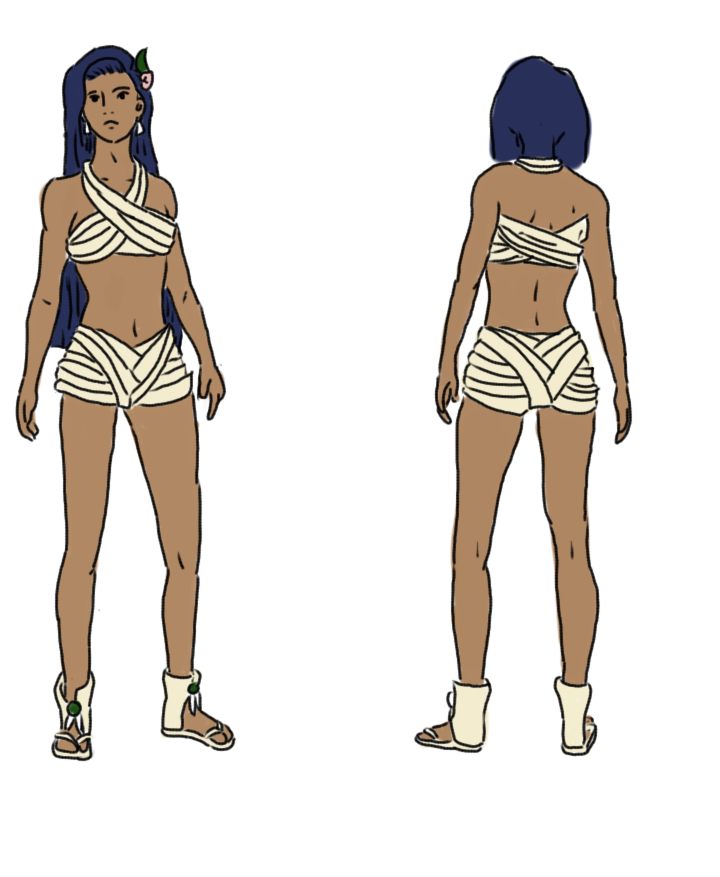
\includegraphics[height=0.3 \textheight]{Imagenes/malinalli}
				\caption{Concepto de diseño de Malinalli.}
				\label{fig:MalinalliDiseno}
\end{figure}
\subsection{Concepto:}
\begin{itemize}
	\item \textbf{Historia antes del juego:}
	Hija del cacique de Oluta. Gracias a su posición social y a la educación recibida de su padre Malinalli fue capaz de aprender y de desarrollar habilidades que cualquier otra niña de su edad no habría podido al ser consideradas como propias de los hombres. Con la muerte de su padre y el segundo matrimonio de su madre, Malinalli es vendida como esclava sin que su madre hiciera algo por impedirlo. Esto causaría en Malinalli un fuerte impacto, impidiéndole a futuro poder confiar en los demás.
	\item \textbf{Historia durante el juego:}
	Los años de esclavitud logran en Malinalli una pérdida de confianza. Malinalli se percibe a si misma como débil e incapaz de hacer un cambio significativo. Desde la perspectiva de Malinalli, su papel se limita a lograr la resurrección de su padre para que él sea quien derrote al imperio y libere a su gente.
	\\
	\par 
	Al principio del juego, Malinalli se mostrará callada y medianamente abierta a mostrar sus emociones. Conforme el viaje avanza, Malinalli se irá volverá más decidida y fuerte. En un principio su motivación será revivir a su padre, pero en algún punto del juego se dará cuenta de que dicha tarea es imposible por lo que su nueva meta será destruir al imperio Mexica para unificar todos los territorios y crear el ombligo de la Luna. Cuando el viaje termine, Malinalli habrá comprendido que para cumplir sus objetivos deberá adaptarse y tener más de mil caras dependiendo de la situación.
	
	\item \textbf{Relaciones:}
	\begin{itemize}
		\item \textbf{Tenelpan:} Padre de Malinalli. Es la persona más importante en la vida de Malinalli y a quien más admira (ver apartado \ref{per:tenepal}).
		\item \textbf{Cimatl: } Madre de Malinalli. Malinalli guarda un fuerte odio hacia ella (ver apartado \ref{per:cimatl}).
		\item \textbf{Xólotl:} En un principio no confía en Xólotl pues piensa que él la va a abandonar en cuanto deje de considerarla útil. Cuando Malinalli comprende el poder que tiene sobre el Dios y sus objetivos, su actitud hacia él cambia. Deja de ser desconfiada y se muestra más servicial y amigable. Malinalli es la única que puede aconsejar a Xólotl sobre futuras acciones y posibles aliados; sin embargo, su consejo no es producto de una amistada sino del deseo de manipular al dios para que éste haga lo que le resulta más útil a los objetivos de Malinalli (ver apartado \ref{per:xolotl}). 
	\end{itemize}			  
\end{itemize}


\subsection{Encuentro:}
Es la protagonista del juego y es a través de ella que el jugador verá como está compuesto la dimensión divina y sus problemas. 

\subsection{Habilidades:}
\begin{itemize}
	\item Disparo de tonalli (ver apartado \ref{hab.disparoT}).
	\item Malinalli posee una gran inteligencia y capacidad de planeación. Debido a sus años como esclava está en buena condición para correr y saltar.
\end{itemize} 
\subsection{Armas:}
Caracola (ver apartado \ref{Arma:Caracola}).
\subsection{Ítems:}
\begin{itemize}
	\item Peineta en forma de flor (ver apartado \ref{item:peineta}).
	\item Armadura espiritual (ver apartado \ref{item:armadura}).
\end{itemize}

\subsection{Bloques de animación}
\begin{itemize}
		\item Animación correr.
		\item Animación saltar.
		\item Animación correr con caracola.
		\item Animación saltar con caracola.
		\item Animación normal.
		\item Animación recibir daño.
		\item Animación morir. 
\end{itemize}